\chapter{Neurónové siete}


Neurónová sieť je založená na orientovanom grafe (ako je možné vidieť na obrázku \ref{fig:nn}), je teda zložená z uzlov, ktoré sú spojené orientovanými hranami \citep{rnn:spol}.
Spojenie uzlu $i$ do uzlu $j$ slúži na propagáciu aktivácie $a_i$ z $i$ do $j$.
Každé takéto spojenie má priradenú váhu $w_{i,j}$, ktorá rozhoduje o sile a znamienku spojenia.
Každý uzol má naviac falošný vstup $a_0=1$ s priradenou váhou $w_{0,j}$.
Všetky uzly si potom vypočítajú váženú hodnotu vstupov, pre uzol $j$ je táto hodnota:
$$in_j=\sum^n_{i=0}w_{i,j}a_i$$
Potom sa na výsledok aplikuje aktivačná funkcia g, tým získame výstup z uzlu:
$$a_j=g(in_j)=g\left(\sum^n_{i=0}w_{i,j}a_i\right)$$

\begin{figure} \label{fig:nn}
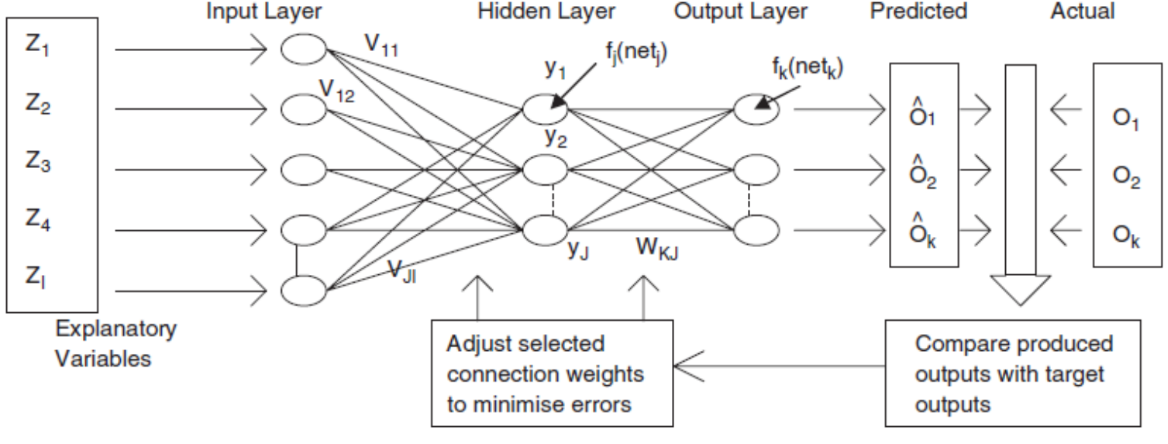
\includegraphics[width=\textwidth]{../img/nn.png}
\caption{Ukážka jednej z neurónových sietí}
\end{figure}

Aktivačná funkcia $g$ je typicky buď pevná hranica alebo logistická funkcia.
V prvom prípade sa uzly volajú perceptrony, v druhom prípade sa niekedy používa pojem sigmoid perceptron.
Obe tieto typy nelineárnych aktivačných funkcií zaručujú dôležitú vlastnosť neurónovej siete, a to, že celá sieť uzlov môže reprezentovať aj nelineárnu funkciu.

\begin{figure}
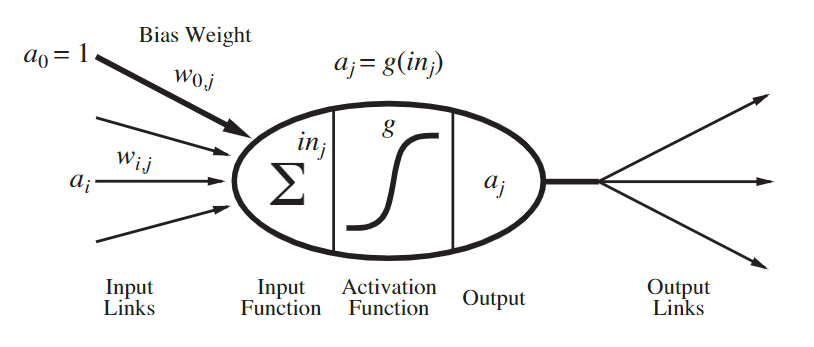
\includegraphics[width=\textwidth]{../img/nn_aima_neuron.png}
\caption{Takto vyzerá jeden uzol siete (neurón) \citep{aima}.}
\end{figure}

Takto teda vyzerá matematický model jedného uzlu (v tomto prípade zvaného neurón) v sieti.
Spájanie týchto neurónov vytvorí sieť.
Existujú dva rozdielne prístupy, akými sa dajú tieto neuróny spojiť do siete. 
Obe nás zaujímajú pre túto prácu, pretože obe použijeme v praxi a budeme ich porovnávať medzi sebou. Tieto prístupy sa nazývajú dopredná a rekuretná neurónová sieť.

\section{Dopredné neurónové siete}
Dopredná neurónová sieť (feed-forward neural network) má spojenia len v jednom smere, takže tvorí orientovaný acyklický graf.
Ak si graf topologicky usporiadame, tak každý uzol dostane vstup z niektorých z predchádzajúcich uzlov a predá výstup niektorým z nasledujúcich vrcholov.
Dopredná neurónová sieť teda predstavuje funkciu jej momentálneho vstupu, teda neuchováva žiaden stav, ak nepočítame váhy samotné.

Tieto siete sú obvykle zoradené do vstiev tak, že každý neurón dostane vstup len z neurónov z predošlej vrstvy.
Podľa počtu vrstiev sa siete delia na jednovrstvové a viacvrstvové \citep{aima}.

\subsection{Jednovrstvové siete}
Jednovrstvové siete spájajú vstupné neuróny priamo s výstupnými.
Tieto siete sú ale obmedzené a nevedia sa naučiť funkcie, ktoré nie sú lineárne separabilné, dokonca aj niektoré jednoduché funkcie ako napríklad XOR \citep{aima}. 

V Euklidovskej geometrii je lineárna separabilita vlastnosť dvoch množín bodov v priestore, ktoré sa dajú presne oddeliť nadrovinou v tomto priestore. 
Najjednoduchšie sa to dá predstaviť v dvojrozmernom priestore napríklad na boolovskej funkcii OR. Bodu (0,0) v súradnicovom systéme (x,y) priradí funkcia hodnotu 0, bodom (1,0), (0,1) a (1,1) priradí hodnotu 1. Ak body rozdelíme do množín podľa priradenej hodnoty, tak tieto dva množiny sa dajú presne oddeliť priamkou, napríklad $y = -x + 1/2$. Je zjavné, že množiny bodov získané z funkcie XOR (tabuľka \ref{xor}) sa takto rozdeliť nedajú, tieto množiny teda nie sú lineárne separabilné.

\begin{table}[h]
\begin{center}
\begin{tabular}{ |c|c|c| } 
 \hline 
 x & y & x XOR y \\ 
 \hline
 0 & 0 & 0 \\ 
 0 & 1 & 1 \\ 
 1 & 0 & 1 \\ 
 1 & 1 & 0 \\ 
 \hline
\end{tabular}
\caption{Tabuľka funkcie XOR}
\label{xor}
\end{center}
\end{table}

\subsection{Viacvrstvové siete}
Viacvrstvové siete majú medzi vstupom do siete a výstupom z nej ešte jednu alebo viac vrstiev tzv. skrytých (hidden) neurónov (Obrázok \ref{img:single}).
Waren McCulloch a Walter Pitts vo svojom článku dokázali, že jeden neurón v sieti vie reprezentovať základné boolovské funkcie AND, OR a NOT a vyslovili, že každá dodatočná funkcionalita sa dá získať spojením väčšieho počtu neurónov do siete \citep{multi}. Samotné XOR z predchádzajúcej podsekcie sa dá vyjadriť ako 
\textit{(x OR y) AND (NOT(x) OR NOT(y))} a podľa tohto vieme vytvoriť aj jednoduchú viacvrstvovú sieť, ktorá používa len neuróny s funkciami AND, OR a NOT (obrázok \ref{img:xor}, matematika týchto viacvrstvových modelov nám však dovoľuje vytvoriť aj jednoduchšie siete pre rozoznávanie XOR, je len potrebné zmeniť aktivačnú funkciu a váhy jednotlivých spojení).

\begin{figure} \label{img:single}
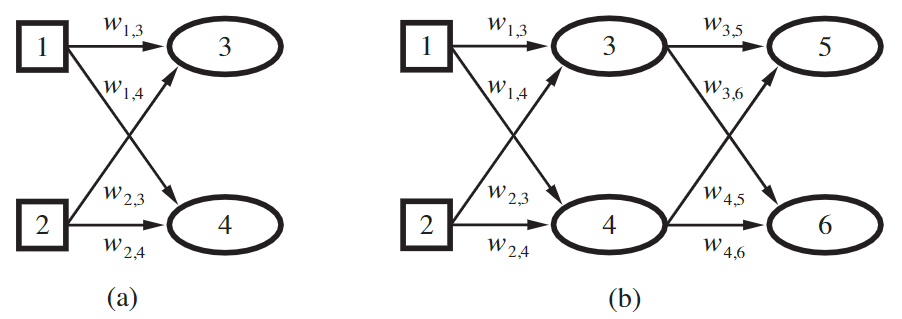
\includegraphics[width=\textwidth]{../img/nn_aima_single_multi.png}
\caption{Ukážka rozdielu medzi jednovrstvou sieťou (a) a viacvrstvovou (b). Obe majú 2 vstupné a 2 výstupné neuróny, viacvrstvová má ešte medzi nimi ďalšie vrstvy skrytých neurónov (v tomto prípade jednu vrstvu s 2 skrytými neurónmi), falošné vstupy do každého neuŕony nie sú ukázané \citep{aima}.}
\end{figure}

\begin{figure} \label{img:xor}
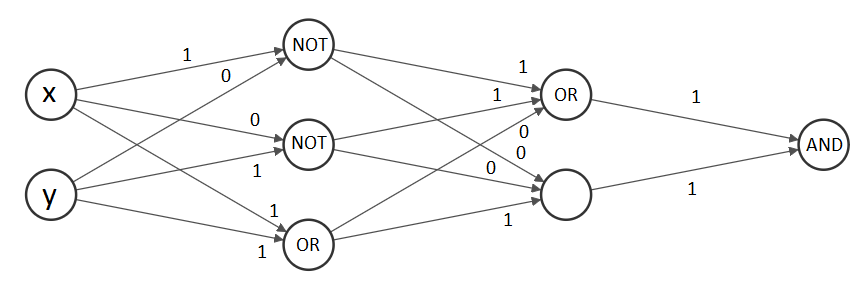
\includegraphics[width=\textwidth]{../img/xor.png}
\caption{Jednoduchá ukážka viacvrstvovej neurónovej siete rozoznávajúcej XOR.}
\end{figure}


\section{Rekurentné neurónové siete}
Na druhej strane je rekurentná neurónová sieť (recurrent neural network).
Tento typ siete posúva svoj výstup naspäť do svojho vlastného vstupu. 
Z toho vyplýva, že aktivačné úrovne siete tvoria dynamický systém, ktorý môže dosiahnuť stabilný stav alebo oscilovať či sa dokonca správať chaoticky.

Výstup siete závisí na vstupe. 
Pri tomto type siete môže výstup závisieť aj na predchádzajúcich výstupoch, tranzitívne teda aj na predchádzajúcich vstupoch.
Z toho vyplýva, že si rekurentná neurónová sieť môže vypracovať krátkodobú pamäť \citep{aima}.

\section{Učenie}
